\section{Results}
\label{sec:results}
We are proving the validity and efficiency of SKBD by evaluating it on two widely used datasets: Structured3D dataset\cite{zheng2020structured3d} and LSUN dataset\cite{zhang2015large}. We are using two standard metrics for evaluation: Corner Error (CE) and Pixel Error (PE). Corner Error is computed by calculating the Euclidean distance between predicted corners and corresponding ground truth corners. Pixel Error is calculated by matching the predicted plane of the floor to the ground truth and calculating a difference as a percentage based on the total number of pixels. For the sake of understandability in \autoref{fig:comparisontest} and \autoref{fig:resultlayouts}, only walls and floors are shown as segments. As SKBD resolves to room layout, the final floor plan has to be calculated by applying a transformation to the polygon associated with the floor for the two methods we are choosing to compare against.

The highlighted algorithms\cite{8451365}\cite{10350607} focus on Room Layout Reconstruction from a single image. However, even in single viewpoint tests our method outperforms these state of the art algorithms. For comparison tests we are choosing two Convolutional Neural Network based approaches, referred to as MC-FCN\cite{8451365} and HGC\cite{10350607}. For MC-FCN, we implemented the model based on the DeepLab-ResNet101\cite{chen2017deeplab} architecture. Both competing models were trained on the training subset of each dataset, respectively.

\begin{figure}[htbp]
\centering
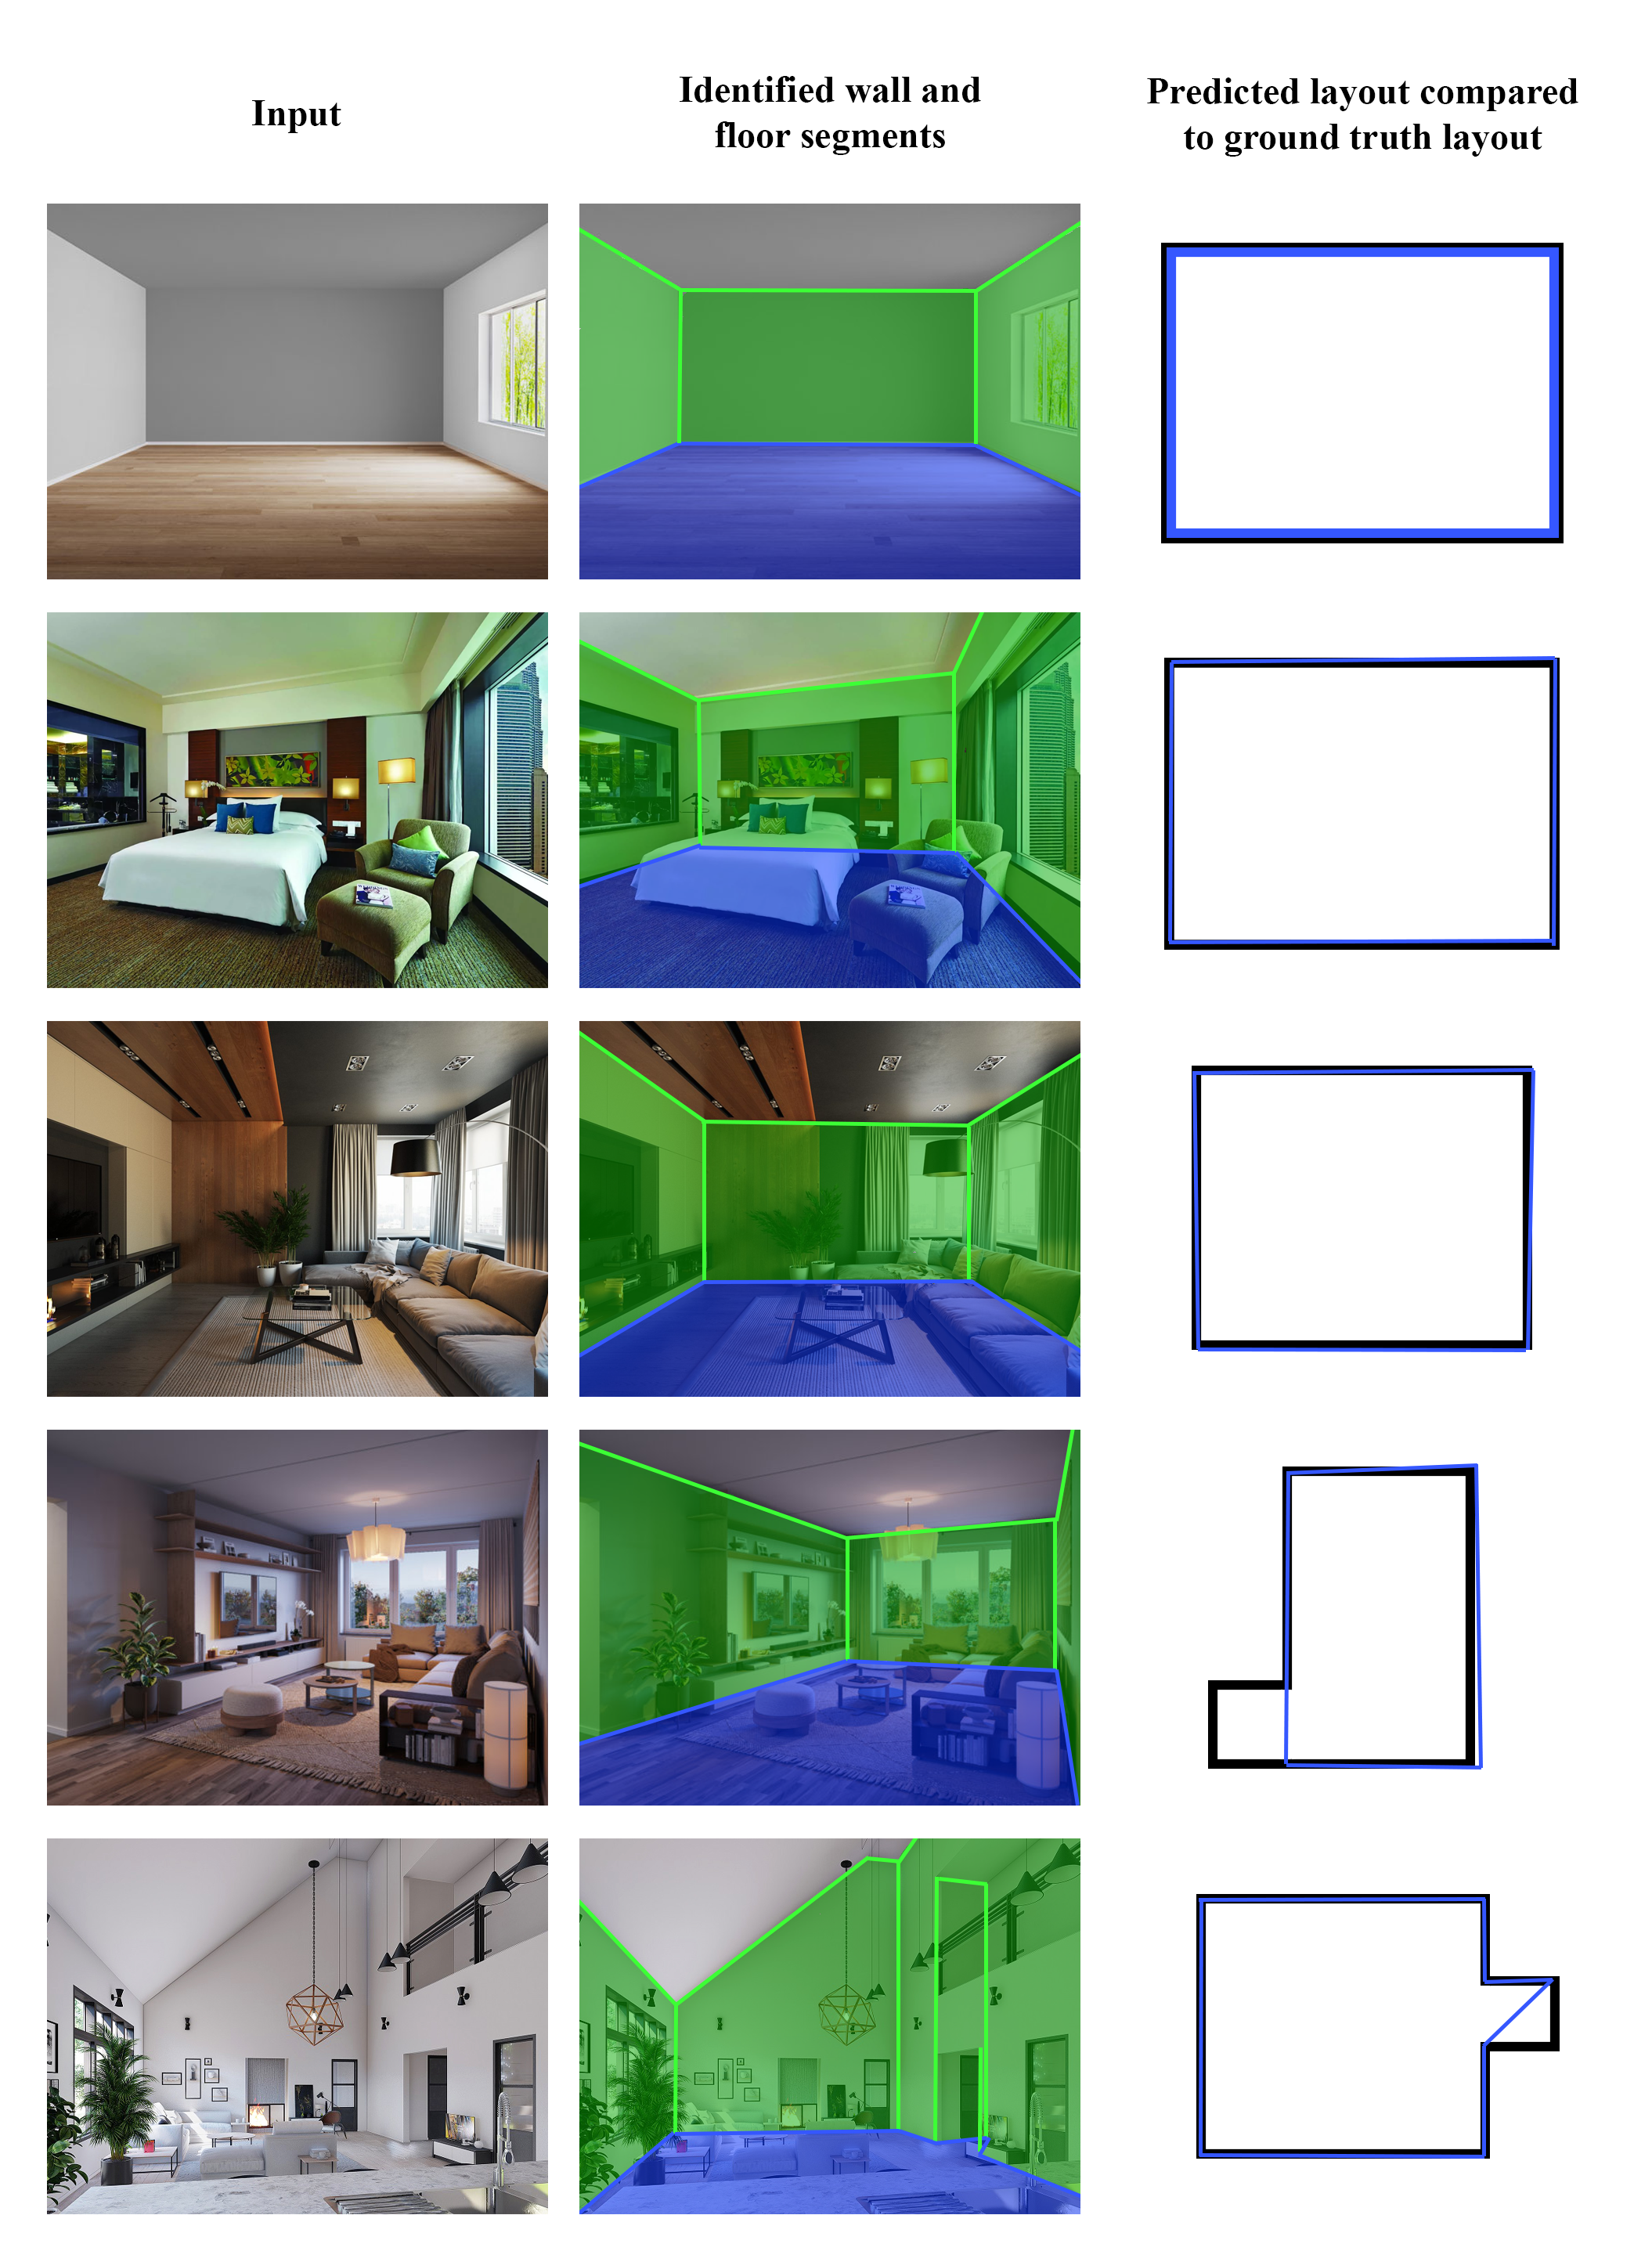
\includegraphics[width=0.9\linewidth]{images/results2.png}
\caption{\label{fig:resultlayouts}Demonstration of the output of SKBD with a few example images taken from Structured3D dataset\cite{zheng2020structured3d} with various levels of clutter and complexity.}
\end{figure}

\begin{figure}[htbp]
\centering
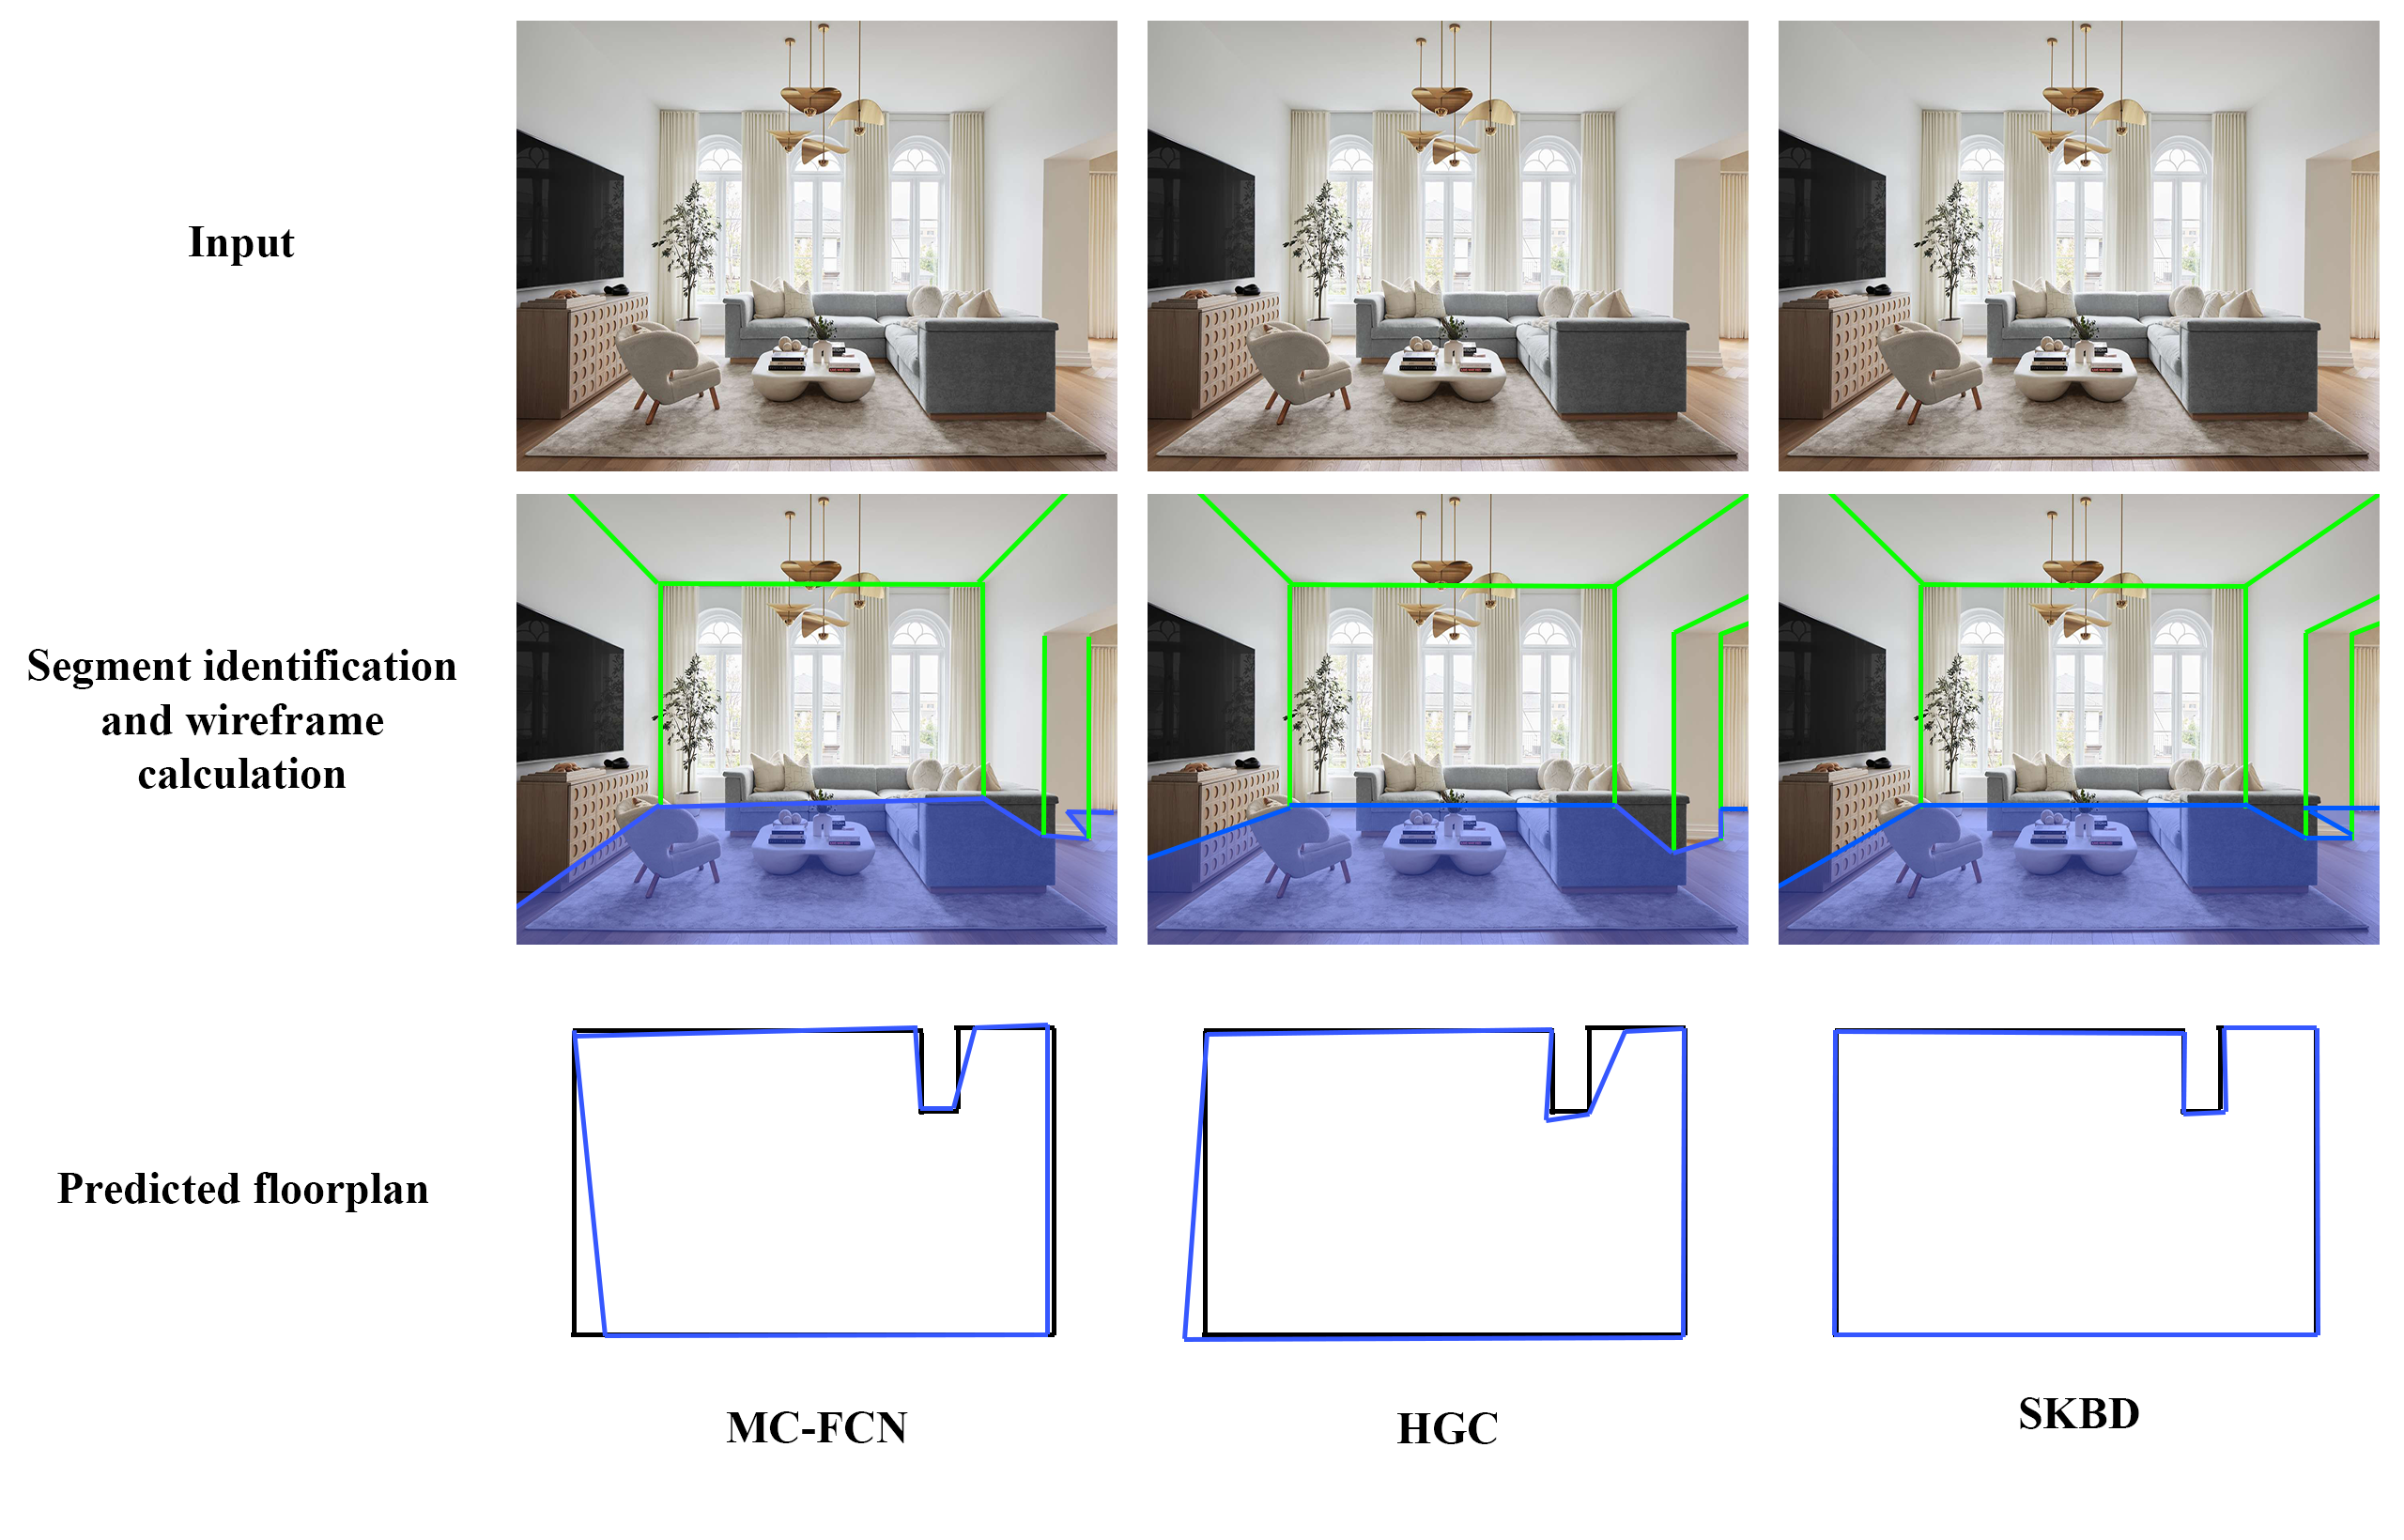
\includegraphics[width=0.9\linewidth]{images/comparison_test_images.png}
\caption{\label{fig:comparisontest}Qualitative test results on an example image taken from Structured3D dataset\cite{zheng2020structured3d} showing successfully identified segments in row two, and a predicted floorplan overlayed on top of the true floorplan in row three.}
\end{figure}

\subsection{Results on Structured3D dataset}
In this test we are using the Strucured3D dataset\cite{zheng2020structured3d}, which is a photo-realistic, large-scale simulated set, containing 3D structure annotations. It consists of 3500 scenes, a total of 21835 rooms and 196515 images, and has a predefined training, validation and test data subset. The input images are resized to \(640 \times 480 \) resolution using bicubic interpolation. For calculating errors, we use the included information about the planes, such as polygon, 3D parameters and semantic label.

Qualitative results are demonstrated in \autoref{fig:comparisontest}. These results also demonstrate that typical FCNs can sometimes be confused by different surfaces and they might generate incorrect wireframes due to occlusions or clutter. Our method works around these uncertainties by utilizing clearly visible segments around said occlusions, and disregarding segments that have a low confidence level. We summarize the results of the test of set Structured3D in \autoref{table:structured3dperf}. SKBD vastly outperforms both algorithms in Pixel Error and Corner Error metrics. Our algorithm is included twice in the test run. The final, highlighted row in \autoref{table:structured3dperf} contains the result of the run where pictures of the same room were grouped together, which allows SKBD to utilize multiple viewpoints for a more accurate and full coverage layout prediction. For fairness, we also include a test run where room grouping was disabled, which causes SKBD to treat each image as a separate room.

This test clearly highlights the key ability of SKBD over other methods, which is combining multiple images to produce a refined and highly accurate floor plan.

\begin{table}[H]
\centering
\begin{tabular}{|c | c c |}
    \hline
    Type & $\epsilon[PE](\%)$ & $\epsilon[CE](\%)$ \\ [0.5 ex]
    \hline\hline
    MC-FCN & 6.91 & 4.98 \\
    HGC & 4.17 & 2.57 \\
    SKBD (single viewpoint) & 1.89 & 1.34 \\
    \hline
    SKBD (multiple viewpoints) & \textbf{0.77} & \textbf{0.68} \\
    \hline
\end{tabular}
\caption{Results on Structured3D dataset}
\label{table:structured3dperf}
\end{table}


\subsection{Results on LSUN dataset}
For this test we are using the relabeled LSUN dataset released by \cite{ren2017coarse}. The dataset consists of 4000 training images, 394 validation images and 1000 testing images. We manually grouped the images taken of the same room from multiple angles, and resized all images to \( 640 \times 480 \) resolution. Ground truth polygon edges and corner points were pre-calculated using the depth and normalmaps included in the dataset, but the input of the algorithms only includes the RGB data. The dataset also provides an official toolkit which suggest the usage of Pixel Error and Corner Error metrics that we also used for the Structured3D set.

This dataset only consists of images of rooms that conform to the Manhattan World Assumption\cite{790349} which favors MC-FCN and HGC. The overall quality of the images are worse compared to the Structured3D set, with more variation in image exposure and more occluions over corners and wall edges. This caused all algorithms to perform worse, however SKBD still outperforms both MC-FCN and HGC as summarized in \autoref{table:lsunperf}.

\begin{table}[H]
\centering
\begin{tabular}{|c | c c |}
    \hline
    Type & $\epsilon[PE](\%)$ & $\epsilon[CE](\%)$ \\ [0.5 ex]
    \hline\hline
    MC-FCN & 8.91 & 6.75 \\
    HGC & 5.29 & 3.44 \\
    SKBD (single viewpoint) & 3.17 & 2.41 \\
    \hline
    SKBD (multiple viewpoints) & \textbf{1.13} & \textbf{1.06} \\
    \hline
\end{tabular}
\caption{Results on LSUN dataset}
\label{table:lsunperf}
\end{table}



